\documentclass[border=5pt]{standalone}
\usepackage{tikz}
\usepackage{amsmath}
\usetikzlibrary{patterns, positioning, decorations.pathreplacing}

\begin{document}

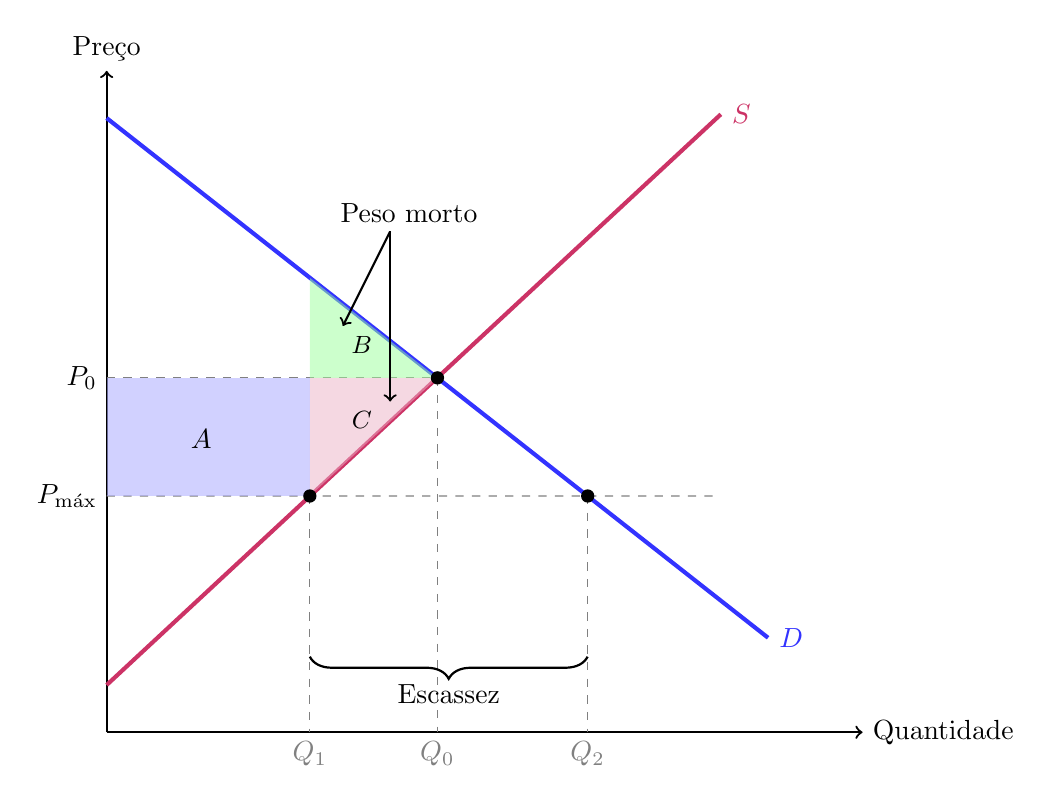
\begin{tikzpicture}[scale=1.2]
    % Eixos
    \draw[thick, ->] (0,0) -- (8,0) node[right] {Quantidade};
    \draw[thick, ->] (0,0) -- (0,7) node[above] {Preço};
    
    % Curva de Demanda (D) - passa por (3.5, 3.75)
    % Equação: y = 6.5 - 0.786*x (passa por (0.5, 6.107) e (3.5, 3.75))
    \draw[thick, blue!80, line width=1.5pt] (0,6.5) -- (7,1) node[right] {$D$};
    
    % Curva de Oferta (S) - passa por (3.5, 3.75)
    % Equação: y = 0.5 + 0.929*x (passa por (0.5, 0.964) e (3.5, 3.75))
    \draw[thick, purple!80, line width=1.5pt] (0,0.5) -- (6.5,6.54) node[right] {$S$};
    
    % Interseção (equilíbrio de mercado)
    \coordinate (E) at (3.5,3.75);
    
    % Preço máximo
    \coordinate (Pmax) at (0,2.5);
    \draw[dashed, gray] (Pmax) -- (6.5,2.5);
    \draw (0,2.5) node[left] {$P_{\text{máx}}$};
    
    % Preço de equilíbrio
    \coordinate (P0) at (0,3.75);
    \draw[dashed, gray] (P0) -- (E);
    \draw (0,3.75) node[left] {$P_0$};
    
    % Quantidades
    \draw[dashed, gray] (2.15,2.5) -- (2.15,0) node[below] {$Q_1$};
    \draw[dashed, gray] (3.5,3.75) -- (3.5,0) node[below] {$Q_0$};
    \draw[dashed, gray] (5.09,2.5) -- (5.09,0) node[below] {$Q_2$};
    
    % Pontos de interseção com Pmáx
    \coordinate (S1) at (2.15,2.5);
    \coordinate (D1) at (5.09,2.5);
    
    % Área A (da origem até Q1, entre Pmáx e P0)
    \fill[blue!30, opacity=0.6] (0,2.5) -- (0,3.75) -- (2.15,3.75) -- (2.15,2.5) -- cycle;
    \node at (1.0,3.1) {$A$};
    
    % Triângulo B (de Q1 até Q0, acima de P0 e abaixo da curva de demanda)
    % Pontos: (2.15, 3.75), (3.5, 3.75), ponto na demanda em Q1
    % Demanda em x=2.15: y = 6.5 - (6.5-1)/7 * 2.15 = 4.81
    \fill[green!40, opacity=0.5] (2.15,3.75) -- (3.5,3.75) -- (2.15,4.81) -- cycle;
    \node at (2.7,4.1) {\small $B$};
    
    % Triângulo C (de Q1 até Q0, acima da curva de oferta e abaixo de P0)
    % Pontos: (2.15, 3.75), (3.5, 3.75), ponto na oferta em Q1
    % Oferta em x=2.15: y = 0.5 + (6.54-0.5)/6.5 * 2.15 = 2.50
    \fill[purple!30, opacity=0.5] (2.15,3.75) -- (3.5,3.75) -- (2.15,2.5) -- cycle;
    \node at (2.7,3.3) {\small $C$};
    
    % Pontos principais
    \fill (E) circle (2pt);
    \fill (S1) circle (2pt);
    \fill (D1) circle (2pt);
    
    % Anotações - Peso morto apontando para B e C
    \node at (3.2,5.5) {Peso morto};
    \draw[->, thick] (3.0,5.3) -- (2.5,4.3);
    \draw[->, thick] (3.0,5.3) -- (3.0,3.5);
    
    % Chave indicando escassez entre Q1 e Q2 (voltada para cima)
    \draw[thick, decoration={brace, amplitude=8pt, mirror}, decorate] (2.15,0.8) -- (5.09,0.8);
    \node at (3.62, 0.4) {Escassez};

\end{tikzpicture}

\end{document}
